\documentclass[12pt, a4paper]{report}

% ===================== PACKAGES =====================
\usepackage{babel}
\babelprovide[import, main]{french}
\usepackage[utf8]{inputenc}
\usepackage[T1]{fontenc}
\usepackage[a4paper, margin=2.5cm]{geometry}
\usepackage{graphicx}
\usepackage{xcolor}
\usepackage{fancyhdr}
\usepackage{titlesec}
\usepackage{longtable}
\usepackage{array}
\usepackage{booktabs}
\usepackage{hyperref}
\usepackage{amsmath}
\usepackage{enumitem}
\usepackage{caption}
\usepackage{tikz}
\usepackage{setspace}
\usepackage{listings}
\usepackage{tabularx}

% ===================== COULEURS =====================
\definecolor{bleuprincipal}{RGB}{16,42,89}
\definecolor{orangeaccent}{RGB}{230,159,0}
\definecolor{codebg}{RGB}{245,245,245}

% ===================== HYPERLINKS =====================
\hypersetup{
    colorlinks=true,
    linkcolor=bleuprincipal,
    citecolor=bleuprincipal,
    urlcolor=bleuprincipal,
    pdftitle={Application École Excellence},
    pdfauthor={Groupe Projet BD}
}

% ===================== EN-TETES / PIEDS DE PAGE =====================
\pagestyle{fancy}
\fancyhf{}
\fancyhead[L]{\small Application École Excellence}
\fancyhead[R]{\small \leftmark}
\fancyfoot[C]{\thepage}
\renewcommand{\headrulewidth}{0.4pt}

% ===================== TITRES DE CHAPITRE =====================
\titleformat{\chapter}[display]
  {\normalfont\bfseries}
  {\Large\chaptertitlename\ \thechapter}
  {10pt}
  {\Huge\color{bleuprincipal}}
\titlespacing*{\chapter}{0pt}{-20pt}{20pt}

\setlength{\parindent}{0pt}
\setlength{\parskip}{6pt}

% ===================== STYLE CODE =====================
\lstset{
    backgroundcolor=\color{codebg},
    basicstyle=\ttfamily\small,
    breaklines=true,
    frame=single,
    columns=fullflexible,
    keepspaces=true,
    captionpos=b
}

\begin{document}

% =====================================================
% TABLE DES MATIERES / FIGURES / TABLEAUX
% =====================================================
\tableofcontents

\listoffigures
\addcontentsline{toc}{chapter}{Liste des figures}

\listoftables
\addcontentsline{toc}{chapter}{Liste des tableaux}

% =====================================================
% INTRODUCTION GENERALE
% =====================================================
\chapter*{Introduction Générale}
\addcontentsline{toc}{chapter}{Introduction Générale}

Au cours des dernières décennies, les technologies de l'information et de la communication ont profondément transformé les méthodes de gestion et d'organisation dans de nombreux secteurs d'activité. Les domaines de la santé, de la finance, du commerce et de l'administration publique ont progressivement adopté des solutions numériques permettant d'améliorer la qualité des services, d'optimiser les processus internes et de faciliter l'accès à l'information. Le secteur de l'éducation s'inscrit aujourd'hui dans cette même dynamique de transformation numérique.

Dans de nombreux établissements scolaires, particulièrement dans les écoles maternelles et primaires des pays en développement, les activités administratives et pédagogiques reposent encore largement sur des méthodes manuelles. Les inscriptions sont souvent réalisées sur support papier, les dossiers des élèves sont archivés physiquement et les notes sont enregistrées dans des registres dont la consultation demeure complexe. Ces pratiques présentent plusieurs limites : perte ou détérioration des documents, redondance des informations, difficultés de recherche dans les archives et délais importants dans le traitement des opérations administratives.

Au Cameroun, cette situation reste observable dans de nombreux établissements. Les responsables administratifs sont confrontés quotidiennement à des difficultés liées à la gestion des élèves, au suivi pédagogique, à la communication avec les parents et à la production des documents académiques. L'absence d'outils numériques adaptés entraîne une surcharge de travail administratif et réduit l'efficacité globale du fonctionnement des établissements.

C'est dans cette perspective que s'inscrit le projet \textbf{« École Excellence »} -- une plateforme web de gestion intégrée destinée aux écoles maternelles et primaires. Cette solution permet la gestion centralisée des élèves, des enseignants, des parents, des classes, des emplois du temps, des notes, des bulletins, des paiements, de la bibliothèque et de la messagerie interne.

L'application repose sur une architecture client-serveur moderne utilisant \textbf{React 19} avec \textbf{TypeScript} et \textbf{Vite} pour le frontend, \textbf{Node.js} avec \textbf{Express 5} et \textbf{TypeScript} pour le backend, et \textbf{PostgreSQL} via \textbf{Prisma ORM} pour la persistance des données. Trois rôles utilisateurs sont définis : \texttt{ADMIN\_PRINCIPAL}, \texttt{PERSONNEL} et \texttt{PARENT}.

Le présent rapport présente l'ensemble des travaux réalisés dans le cadre de ce projet. Il est structuré en plusieurs chapitres : le premier présente le contexte et les objectifs ; le deuxième détaille l'analyse des besoins ; le troisième décrit la conception du système ; le quatrième expose la réalisation et l'implémentation ; les derniers chapitres sont consacrés aux tests, aux difficultés rencontrées et aux perspectives.

% =====================================================
% CHAPITRE 1 : PRÉSENTATION DU PROJET
% =====================================================
\chapter{Présentation du Projet}

\section{Introduction}
L'évolution des technologies numériques a profondément modifié les méthodes de gestion dans de nombreux secteurs d'activité. Le domaine de l'éducation connaît progressivement une transition vers des solutions informatiques permettant d'améliorer l'efficacité des processus administratifs et pédagogiques.

Dans cette optique, nous avons conçu et développé \textbf{École Excellence}, une application web destinée à la gestion des écoles maternelles et primaires. Ce projet vise à proposer une solution moderne permettant de centraliser les informations scolaires, de simplifier les opérations administratives et de renforcer la communication entre les différents acteurs de l'établissement.

\section{Contexte du projet}
Les établissements scolaires maternels et primaires sont confrontés quotidiennement à la gestion d'un volume important d'informations relatives aux élèves, aux enseignants, aux parents, aux classes, aux évaluations et aux opérations financières.

Dans de nombreux établissements, ces activités sont encore réalisées à l'aide de registres papier ou de fichiers bureautiques dispersés. Cette situation engendre plusieurs difficultés :
\begin{itemize}[noitemsep]
    \item perte ou détérioration des informations ;
    \item duplication des données ;
    \item erreurs de saisie ;
    \item difficulté d'accès aux informations historiques ;
    \item temps important consacré aux tâches administratives ;
    \item communication limitée avec les parents d'élèves.
\end{itemize}

\section{Problématique}
La gestion manuelle des établissements scolaires présente de nombreuses limites qui impactent directement l'efficacité des activités administratives et pédagogiques. Les responsables d'établissement doivent gérer simultanément les inscriptions des élèves, le suivi des enseignants, la gestion des notes, la production des bulletins scolaires, le suivi des paiements ainsi que l'organisation du transport scolaire.

La problématique principale peut être formulée comme suit :

\begin{quote}
\itshape Comment concevoir et développer une application web centralisée permettant d'assurer une gestion efficace, sécurisée et moderne des activités administratives et pédagogiques des écoles maternelles et primaires ?
\end{quote}

\section{Objectifs du projet}

\subsection{Objectif général}
Concevoir et développer une application web permettant d'automatiser et de centraliser la gestion administrative, pédagogique et financière des écoles maternelles et primaires.

\subsection{Objectifs spécifiques}
\begin{itemize}[noitemsep]
    \item gérer les informations relatives aux élèves ;
    \item gérer les informations des parents ;
    \item gérer les enseignants et le personnel ;
    \item administrer les classes, cycles et matières ;
    \item faciliter la saisie et la consultation des notes ;
    \item générer automatiquement les bulletins scolaires en PDF ;
    \item assurer le suivi des paiements scolaires ;
    \item gérer la bibliothèque numérique ;
    \item planifier les emplois du temps ;
    \item permettre la messagerie interne avec modération ;
    \item garantir la sécurité et la confidentialité des données.
\end{itemize}

\section{Présentation de la solution proposée}
La solution développée est une application web accessible via un navigateur, organisée en trois espaces distincts correspondant aux trois profils d'utilisateurs :

\begin{itemize}[noitemsep]
    \item \textbf{Espace Admin Principal} : tableau de bord, gestion des inscriptions, des élèves, du personnel, des matières, des salles, des plannings, des bulletins, des paiements, de la bibliothèque, de la discipline et de la configuration académique.
    \item \textbf{Espace Enseignant} : consultation des cours assignés, saisie des notes, dépôt d'épreuves, signalement d'incidents, messagerie aux parents.
    \item \textbf{Espace Parent} : suivi des enfants (bulletins, discipline, planning), paiement des frais de scolarité, consultation de la bibliothèque.
\end{itemize}

\section{Technologies utilisées}
L'application repose sur une architecture moderne basée sur les technologies suivantes :

\begin{table}[htbp]
\centering
\small
\begin{tabular}{|p{3.5cm}|p{3cm}|p{7cm}|}
\hline
\textbf{Composant} & \textbf{Technologie} & \textbf{Rôle} \\
\hline
Interface utilisateur & React 19 + TypeScript + Vite & Développement de l'interface utilisateur côté client \\
\hline
Styles & Tailwind CSS 4 & Mise en page responsive et moderne \\
\hline
Serveur applicatif & Node.js + Express 5 + TypeScript & API REST, logique métier, authentification \\
\hline
Base de données & PostgreSQL + Prisma ORM & Persistance des données et migrations \\
\hline
Authentification & JWT (jsonwebtoken + bcrypt) & Génération et vérification des tokens \\
\hline
Génération PDF & jsPDF + jspdf-autotable & Bulletins et factures \\
\hline
Paiements & Orange Money / MTN MoMo / Carte bancaire & Intégration des moyens de paiement \\
\hline
Déploiement frontend & Vercel & Hébergement de l'interface React \\
\hline
Déploiement backend & Railway & Hébergement du serveur Node.js \\
\hline
\end{tabular}
\caption{Technologies utilisées}
\label{tab:technologies}
\end{table}

\section{Organisation de l'équipe}
La réalisation du projet a mobilisé une équipe composée de huit membres travaillant de manière collaborative afin d'assurer le respect des objectifs fixés et des délais impartis.

\section{Méthodologie de travail}
Nous avons adopté une démarche de développement incrémentale, découpée en plusieurs phases :
\begin{enumerate}[noitemsep]
    \item Analyse des besoins ;
    \item Conception du système (UML) ;
    \item Conception de la base de données (Prisma) ;
    \item Développement du backend (API REST) ;
    \item Développement du frontend (React) ;
    \item Intégration des modules ;
    \item Tests et validation ;
    \item Documentation du projet.
\end{enumerate}

\section{Conclusion}
Ce chapitre a présenté le contexte général du projet, les problèmes identifiés, les objectifs poursuivis ainsi que l'organisation adoptée. L'analyse détaillée des besoins fonctionnels et non fonctionnels sera présentée dans le chapitre suivant.

% =====================================================
% CHAPITRE 2 : EXPRESSION DES BESOINS
% =====================================================
\chapter{Expression des besoins}

L'expression des besoins consiste à identifier les fonctionnalités attendues par les différents utilisateurs de l'application ainsi que les contraintes que le système doit respecter. Cette étape permet de définir clairement les services que l'application devra fournir.

\section{Identification des acteurs du système}
Un acteur représente une entité qui interagit avec le système. Dans l'application École Excellence, les principaux acteurs sont :

\subsection{Administrateur principal (\texttt{ADMIN\_PRINCIPAL})}
Responsable de la gestion globale de l'établissement. Il dispose des droits les plus étendus :
\begin{itemize}[noitemsep]
    \item valider les comptes en attente ;
    \item gérer les élèves (CRUD) ;
    \item gérer le personnel (enseignants, surveillants, secrétaires) ;
    \item créer et configurer les classes, cycles et matières ;
    \item affecter les enseignants aux salles (promotion titulaire) ;
    \item planifier les emplois du temps ;
    \item générer les bulletins scolaires ;
    \item valider les paiements et configurer les frais de scolarité ;
    \item gérer la bibliothèque ;
    \item modérer les messages des enseignants ;
    \item configurer les années académiques, trimestres et sessions ;
    \item gérer la discipline (types d'infractions, incidents).
\end{itemize}

\subsection{Personnel enseignant (\texttt{PERSONNEL})}
Chargé du suivi pédagogique des élèves qui lui sont affectés :
\begin{itemize}[noitemsep]
    \item consulter les cours assignés et les élèves ;
    \item saisir les notes (individuelle ou groupée) ;
    \item déposer des épreuves (PDF) ;
    \item signaler des incidents disciplinaires ;
    \item envoyer des messages aux parents de sa classe (avec modération) ;
    \item consulter son emploi du temps.
\end{itemize}

\subsection{Parent d'élève (\texttt{PARENT})}
Utilisateur externe chargé du suivi scolaire de ses enfants :
\begin{itemize}[noitemsep]
    \item soumettre une demande d'inscription ;
    \item consulter les bulletins et notes ;
    \item suivre la discipline ;
    \item consulter l'emploi du temps ;
    \item effectuer des paiements ;
    \item consulter la bibliothèque.
\end{itemize}

\section{Besoins fonctionnels}

\subsection{Gestion des utilisateurs et authentification}
Le système doit permettre :
\begin{itemize}[noitemsep]
    \item l'inscription avec statut \texttt{PENDING} en attente de validation ;
    \item la connexion sécurisée par email et mot de passe (bcrypt + JWT) ;
    \item la gestion des rôles (\texttt{ADMIN\_PRINCIPAL}, \texttt{PERSONNEL}, \texttt{PARENT}) ;
    \item l'activation / désactivation des comptes.
\end{itemize}

\subsection{Gestion des inscriptions}
L'application doit permettre aux parents de soumettre une demande d'inscription avec photo de l'enfant, et à l'administrateur de l'approuver ou la rejeter.

\subsection{Gestion des élèves}
\begin{itemize}[noitemsep]
    \item enregistrement, modification, suppression ;
    \item consultation par classe ;
    \item upload de photo administrateur ;
    \item suivi du statut (inscrit, actif, etc.).
\end{itemize}

\subsection{Gestion pédagogique}
\begin{itemize}[noitemsep]
    \item création et gestion des cycles, classes et matières ;
    \item affectation des enseignants aux classes ;
    \item planification des emplois du temps par classe et par salle ;
    \item saisie des notes avec évaluation ;
    \item génération des bulletins PDF avec moyennes, classement et assiduité.
\end{itemize}

\subsection{Gestion financière}
\begin{itemize}[noitemsep]
    \item configuration des frais de scolarité par classe ;
    \item définition des tranches de paiement ;
    \item enregistrement des paiements (Orange Money, MTN MoMo, carte bancaire) ;
    \item validation des paiements par l'administrateur.
\end{itemize}

\subsection{Messagerie interne}
\begin{itemize}[noitemsep]
    \item envoi d'annonces par l'administrateur à tous les parents ;
    \item messages personnels administrateur $\rightarrow$ parent ;
    \item messages enseignant $\rightarrow$ parents de sa classe (statut \texttt{PENDING}) ;
    \item modération des messages par l'administrateur.
\end{itemize}

\subsection{Gestion de la bibliothèque}
\begin{itemize}[noitemsep]
    \item ajout, modification et suppression de livres ;
    \item upload de couverture et de fichier PDF ;
    \item consultation par les parents et enseignants.
\end{itemize}

\subsection{Discipline}
\begin{itemize}[noitemsep]
    \item signalement d'incidents (retard, absence, comportement) ;
    \item système de points avec malus ;
    \item types d'infractions paramétrables.
\end{itemize}

\subsection{Gestion académique}
\begin{itemize}[noitemsep]
    \item création des années académiques ;
    \item génération des trimestres et sessions d'évaluation ;
    \item duplication d'une année.
\end{itemize}

\section{Besoins non fonctionnels}

\subsection{Sécurité}
\begin{itemize}[noitemsep]
    \item mots de passe hashés avec bcrypt ;
    \item authentification par JWT (token expirant) ;
    \item middleware de protection des routes (`protect`) ;
    \item restriction d'accès par rôle (`restrictTo`) ;
    \item protection contre les injections SQL via Prisma.
\end{itemize}

\subsection{Ergonomie}
\begin{itemize}[noitemsep]
    \item interface responsive adaptée aux mobiles et tablettes ;
    \item navigation intuitive avec layout adapté à chaque rôle ;
    \item support multilingue (français / anglais).
\end{itemize}

\subsection{Performance}
\begin{itemize}[noitemsep]
    \item temps de réponse rapide pour les opérations courantes ;
    \item génération asynchrone des bulletins ;
    \item pagination des listes d'élèves.
\end{itemize}

\subsection{Adaptation au contexte camerounais}
\begin{itemize}[noitemsep]
    \item paiement en plusieurs tranches (scolarité adaptée) ;
    \item cycles SIL, CP, CE1, CE2, CM1, CM2 ;
    \item modes de paiement locaux (Orange Money, MTN MoMo).
\end{itemize}

% =====================================================
% CHAPITRE 3 : CONCEPTION DU SYSTÈME
% =====================================================
\chapter{Conception du système}

La conception du système consiste à définir l'architecture générale de la solution, les différents composants ainsi que les interactions entre les acteurs et l'application. Cette phase permet de transformer les besoins exprimés en une représentation technique facilitant l'implémentation.

\section{Architecture générale de l'application}
L'application École Excellence repose sur une architecture en couches permettant de séparer les différentes responsabilités du système :

\begin{table}[htbp]
\centering
\small
\begin{tabular}{|p{2.8cm}|p{5cm}|p{5cm}|}
\hline
\textbf{Couche} & \textbf{Rôle} & \textbf{Composants associés} \\
\hline
Couche présentation & Interface utilisateur React & Pages admin, enseignant, parent ; formulaires ; tableaux de bord \\
\hline
Couche API & Routes et middlewares Express & 20 routeurs REST ; middleware auth ; validation \\
\hline
Couche métier & Contrôleurs et logique applicative & 20 contrôleurs ; calculs ; génération PDF \\
\hline
Couche données & ORM Prisma + PostgreSQL & Modèles, migrations, requêtes préparées \\
\hline
\end{tabular}
\caption{Architecture en couches d'École Excellence}
\label{tab:archi_couches}
\end{table}

\section{Architecture fonctionnelle}

\begin{table}[htbp]
\centering
\small
\begin{tabular}{|p{2.5cm}|p{4cm}|p{7cm}|}
\hline
\textbf{Acteur} & \textbf{Espace} & \textbf{Fonctionnalités principales} \\
\hline
Admin principal & Administration & Dashboard, inscriptions, élèves, personnel, matières, salles, plannings, bulletins, paiements, bibliothèque, discipline, messagerie, configuration académique \\
\hline
Enseignant & Pédagogie & Cours, notes, épreuves, discipline, messagerie, planning \\
\hline
Parent & Suivi familial & Inscriptions, bulletins, discipline, planning, paiements, bibliothèque, scolarité \\
\hline
\end{tabular}
\caption{Architecture fonctionnelle}
\label{tab:archi_fonctionnelle}
\end{table}

\section{Modélisation UML du système}

\subsection{Diagramme de cas d'utilisation}
Le diagramme de cas d'utilisation présente les interactions entre les acteurs et les fonctionnalités du système.

\begin{figure}[htbp]
    \centering
    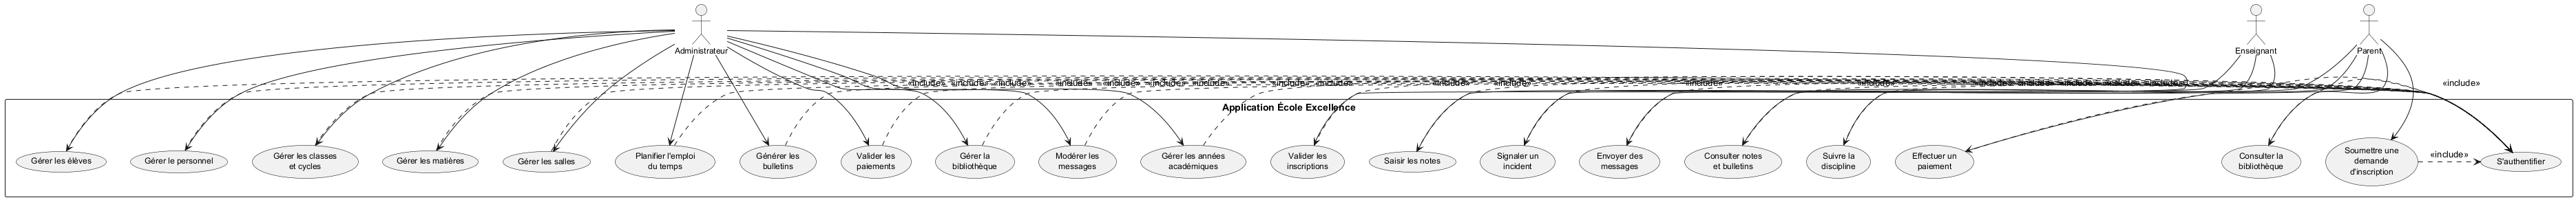
\includegraphics[width=\textwidth]{images/diagramme_cas_utilisation.png}
    \caption{Diagramme des cas d'utilisation}
    \label{fig:cas_utilisation}
\end{figure}

\subsection{Diagramme de classes}
Le diagramme de classes représente la structure statique du système avec les principales entités et leurs relations.

\begin{figure}[htbp]
    \centering
    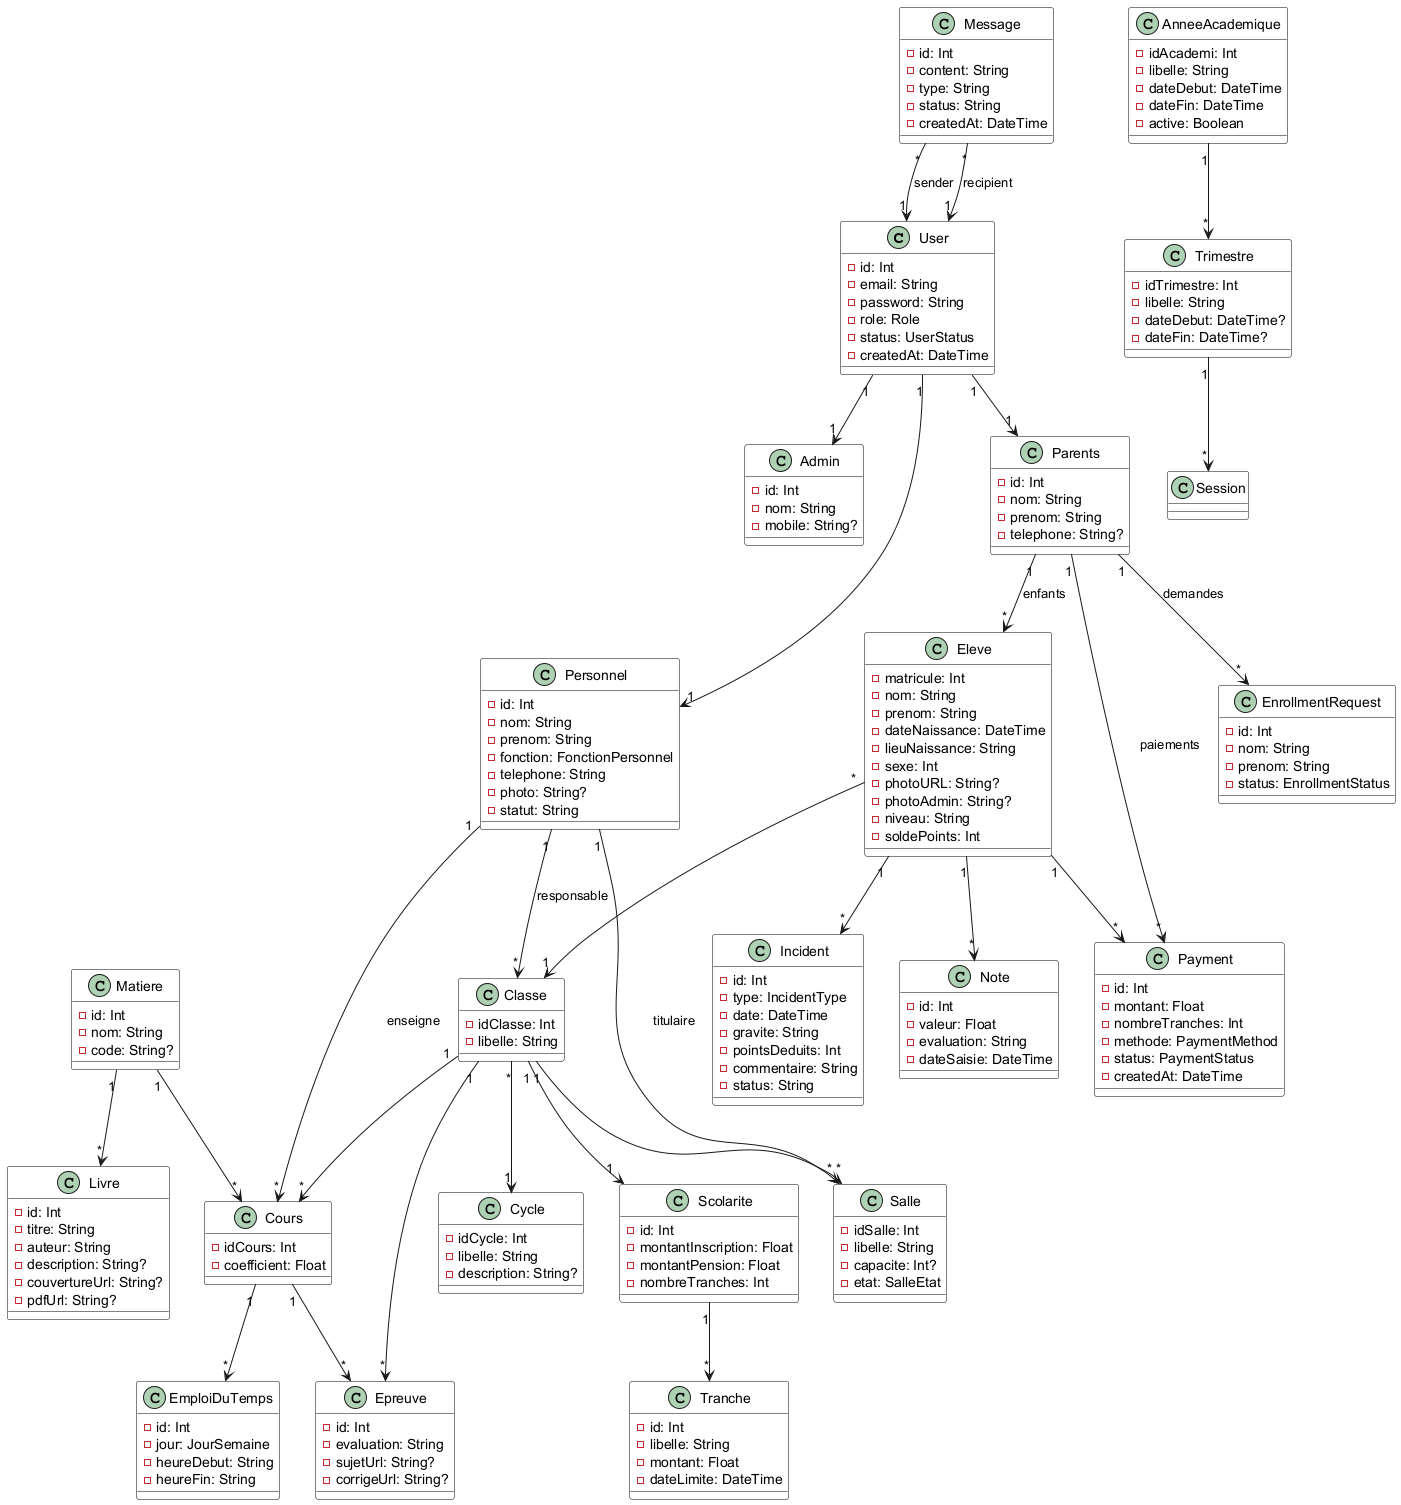
\includegraphics[width=\textwidth]{images/diagramme_classes.png}
    \caption{Diagramme de classes}
    \label{fig:classes}
\end{figure}

\subsection{Diagramme de séquence -- Authentification}

\begin{figure}[htbp]
    \centering
    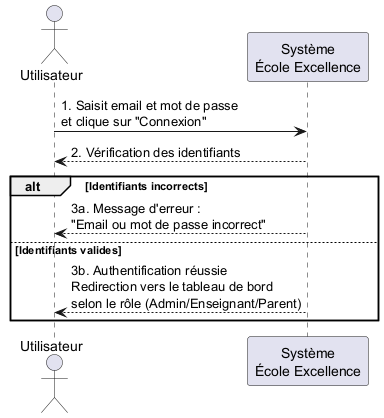
\includegraphics[width=\textwidth]{images/seq_systeme_authentification.png}
    \caption{Diagramme de séquence système -- Authentification}
    \label{fig:seq_auth}
\end{figure}

\subsection{Diagramme de séquence -- Inscription d'un élève}

\begin{figure}[htbp]
    \centering
    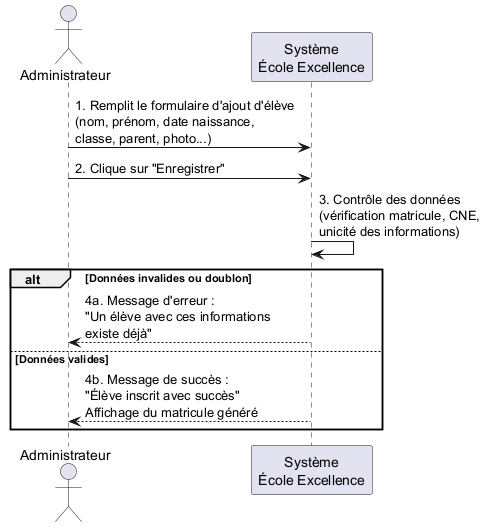
\includegraphics[width=\textwidth]{images/seq_systeme_ajout_eleve.png}
    \caption{Diagramme de séquence système -- Ajout d'un élève}
    \label{fig:seq_eleve}
\end{figure}

\subsection{Diagramme de séquence -- Paiement}

\begin{figure}[htbp]
    \centering
    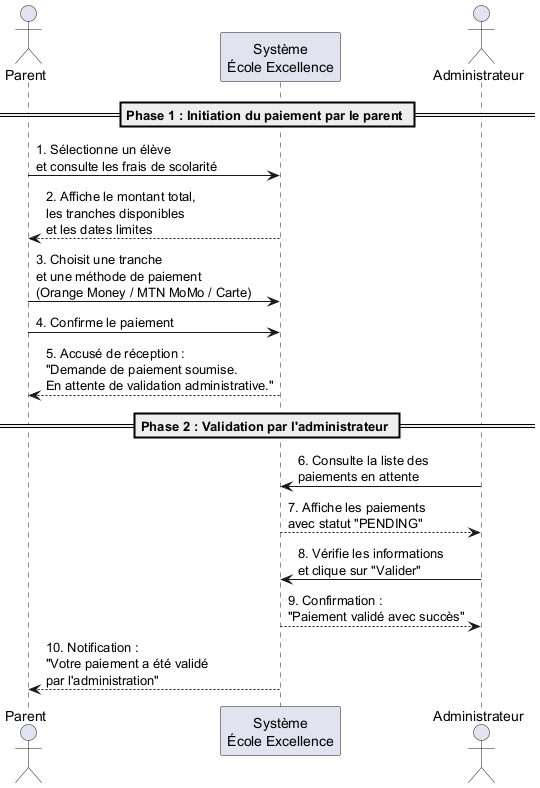
\includegraphics[width=\textwidth]{images/seq_systeme_paiement.png}
    \caption{Diagramme de séquence système -- Paiement de frais scolaires}
    \label{fig:seq_paiement}
\end{figure}

\section{Modèle de données}

Le modèle de données est défini via le schéma Prisma et comporte 27 modèles principaux :

\begin{longtable}{|p{3cm}|p{4cm}|p{6.5cm}|}
\hline
\textbf{Modèle} & \textbf{Clé primaire} & \textbf{Description} \\
\hline
\endhead
\hline
\endfoot
User & id & Table centrale d'authentification (email, password, role, status) \\
Admin & id & Profil administrateur \\
Personnel & id & Profil personnel (nom, fonction, téléphone, photo) \\
Parents & id & Profil parent \\
Eleve & matricule & Élève (nom, prénom, date naissance, classe, photo) \\
Classe & idClasse & Classe (libellé, cycle, responsable) \\
Cycle & idCycle & Cycle pédagogique (SIL, CP, CE, CM) \\
Salle & idSalle & Salle de classe (libellé, capacité, état) \\
Matiere & id & Matière enseignée \\
MatiereClasse & (matiere, classe) & Association matière-classe \\
Cours & idCours & Cours (matière, classe, enseignant, salle, coefficient) \\
Note & id & Note (valeur, évaluation, matière, élève) \\
Evaluation & idEval & Évaluation (note, appréciation, cours, élève) \\
Incident & id & Incident disciplinaire (type, gravité, points, élève) \\
TypeInfraction & id & Catalogue d'infractions paramétrables \\
EmploiDuTemps & id & Créneau planning (jour, heure, cours, salle) \\
Payment & id & Paiement (montant, méthode, statut, élève, parent) \\
Scolarite & id & Configuration frais par classe (montant, tranches) \\
Tranche & id & Tranche de paiement (libellé, montant, date limite) \\
Livre & id & Livre de bibliothèque (titre, auteur, cycle, PDF) \\
Message & id & Message (contenu, type, statut, expéditeur, destinataire) \\
Epreuve & id & Épreuve (évaluation, sujet, corrigé, matière, classe) \\
AnneeAcademique & idAcademi & Année scolaire (libellé, dates, statut) \\
Trimestre & idTrimestre & Trimestre (libellé, dates, année) \\
Session & idSession & Session d'évaluation (trimestre) \\
Frequente & idFrequente & Fréquentation élève-classe-année \\
EnrollmentRequest & id & Demande d'inscription (statut, parent) \\
FeeConfig & id & Configuration des frais par niveau \\
ProcedureInscription & id & Procédure d'inscription (contenu HTML) \\
\hline
\caption{Modèles de données de l'application}
\label{tab:modeles}
\end{longtable}

% =====================================================
% CHAPITRE 4 : RÉALISATION ET IMPLÉMENTATION
% =====================================================
\chapter{Réalisation et implémentation}

\section{Introduction}
Après l'analyse des besoins et la conception du système, cette phase consiste à mettre en œuvre les différentes fonctionnalités en utilisant les technologies définies précédemment. Cette section présente l'organisation du code source, l'architecture détaillée, les principaux modules et la structure de la base de données.

\section{Environnement de développement}

\begin{table}[htbp]
\centering
\small
\begin{tabular}{|p{3cm}|p{3cm}|p{7cm}|}
\hline
\textbf{Outil} & \textbf{Type} & \textbf{Utilisation} \\
\hline
Visual Studio Code & Éditeur de code & Développement du code source \\
\hline
GitHub & Gestion de versions & Stockage du code et collaboration \\
\hline
Overleaf & Rédaction LaTeX & Rédaction collaborative du rapport \\
\hline
Vercel & Déploiement frontend & Hébergement de l'interface React \\
\hline
Railway & Déploiement backend & Hébergement du serveur Node.js \\
\hline
Supabase & Base de données & Hébergement PostgreSQL \\
\hline
\end{tabular}
\caption{Environnement de développement}
\label{tab:env_dev}
\end{table}

\section{Architecture du backend}

Le backend de l'application École Excellence est construit avec \textbf{Node.js} et \textbf{Express 5} en \textbf{TypeScript}. Il suit une architecture modulaire organisée autour de quatre dossiers principaux dans \texttt{src/}.

Le dossier \texttt{controllers/} contient la logique métier répartie dans 20 fichiers, chacun responsable d'un domaine fonctionnel : authentification, administration, inscriptions, élèves, bulletins, notes, discipline, planning, cours, matières, personnel, salles, paiements, bibliothèque, messages, épreuves, gestion académique, procédure d'inscription, scolarité et comptes utilisateurs.

Le dossier \texttt{routes/} déclare les endpoints REST. Chacun des 20 routeurs importe le contrôleur correspondant et définit le chemin, la méthode HTTP et les middlewares de protection (authentification JWT et restriction par rôle). L'API expose au total plus de 80 endpoints.

Le dossier \texttt{middlewares/} regroupe les couches transversales : \texttt{authMiddleware.ts} fournit les fonctions \texttt{protect} (vérification du token JWT) et \texttt{restrictTo(...)} (contrôle d'accès par rôle), tandis que les fichiers \texttt{upload*.ts} gèrent les téléversements de fichiers via Multer (photos d'élèves, couvertures et PDFs de livres).

Le dossier \texttt{lib/} contient l'instance unique du client Prisma (pattern singleton), utilisée par tous les contrôleurs pour interagir avec la base de données PostgreSQL.

En complément, le dossier \texttt{prisma/} à la racine du backend définit le schéma de données complet (27 modèles, énums et relations) et contient l'historique des migrations. Le fichier \texttt{seed.ts} initialise la base avec les données de base (comptes administrateur, cycles, classes), tandis que \texttt{scripts/createAdmin.ts} est un utilitaire CLI pour créer un compte administrateur. Un dossier \texttt{uploads/} stocke les fichiers téléchargés (épreuves, livres, photos).

\section{Architecture du frontend}

Le frontend est développé avec \textbf{React 19}, \textbf{TypeScript} et \textbf{Vite}. L'architecture est organisée par fonctionnalité et par rôle utilisateur.

Le point d'entrée \texttt{main.tsx} monte l'application React dans le DOM. \texttt{App.tsx} définit le routeur principal qui structure l'application en trois couches : les providers (contextes), les layouts (un par rôle) et les pages.

Le dossier \texttt{components/} contient les composants réutilisables : des composants transversaux comme \texttt{ProtectedRoute} (garde d'accès par rôle), \texttt{Spinner} (indicateur de chargement), \texttt{LanguageSwitcher} (sélecteur bilingue français/anglais), \texttt{SubmitBtn} et \texttt{ConfirmModal}, ainsi que des sous-dossiers spécialisés par rôle (\texttt{layout/}, \texttt{admin/}, \texttt{teacher/}, \texttt{parent/}).

Le dossier \texttt{pages/} organise les vues selon les trois profils d'utilisateurs : 14 pages pour l'administrateur principal (dashboard, inscriptions, élèves, matières, personnel, salles, plannings, bulletins, paiements, bibliothèque, discipline, messagerie, configuration académique, comptes désactivés), 7 pages pour l'enseignant (dashboard, notes, épreuves, discipline, planning, messagerie, détail cours) et 7 pages pour le parent (profil enfant, bulletins, discipline, planning, paiement, bibliothèque, frais de scolarité).

Le dossier \texttt{services/} configure la couche de communication avec l'API via Axios (\texttt{axiosInstance.ts}) avec intercepteur JWT automatique, et expose des fonctions d'appel organisées par domaine (\texttt{apiServices.ts}, \texttt{enrollmentService.ts}).

Les dossiers \texttt{contexts/}, \texttt{i18n/} et \texttt{types/} gèrent respectivement l'état global React (langue, logo, thème), les fichiers de traduction JSON (français et anglais) et les définitions TypeScript partagées. Enfin, \texttt{utils/} regroupe les utilitaires de génération PDF (bulletins et factures avec jsPDF), les notifications toast et un hook de gestion d'état de chargement.

\section{Architecture de la base de données}

La base de données est hébergée sur Supabase (PostgreSQL). L'ORM Prisma assure la gestion des migrations et l'exécution sécurisée des requêtes.

Le schéma relationnel comprend 27 modèles interconnectés. Voici les relations principales :

\begin{itemize}[noitemsep]
    \item \textbf{User} $\rightarrow$ \texttt{Admin}, \texttt{Personnel}, \texttt{Parents} (1:1)
    \item \textbf{Parents} $\rightarrow$ \texttt{Eleve} (1:N)
    \item \textbf{Eleve} $\rightarrow$ \texttt{Classe} (N:1), \texttt{Note} (1:N), \texttt{Incident} (1:N), \texttt{Payment} (1:N)
    \item \textbf{Classe} $\rightarrow$ \texttt{Cycle} (N:1), \texttt{Cours} (1:N), \texttt{MatiereClasse} (1:N)
    \item \textbf{Personnel} $\rightarrow$ \texttt{Classe} (1:N, responsable), \texttt{Cours} (1:N)
    \item \textbf{Matiere} $\rightarrow$ \texttt{Cours} (1:N), \texttt{Livre} (1:N), \texttt{MatiereClasse} (1:N)
    \item \textbf{AnneAcademique} $\rightarrow$ \texttt{Trimestre} (1:N) $\rightarrow$ \texttt{Session} (1:N)
\end{itemize}

\section{API REST -- Liste des endpoints}

L'API expose plus de 80 endpoints répartis dans 20 routeurs, tous protégés par authentification JWT et restriction par rôle.

\begin{longtable}{|p{2.5cm}|p{3cm}|p{8cm}|}
\hline
\textbf{Module} & \textbf{Préfixe} & \textbf{Endpoints principaux} \\
\hline
\endhead
\hline
\endfoot
Auth & /api/auth & POST register, POST login, GET profile \\
Admin & /api/admin & GET stats, GET/POST salles/matieres/personnel, POST validate \\
Enrollments & /api/enrollments & CRUD demandes, cycles, classes, profils enfants \\
Students & /api/students & CRUD eleves, liste par classe, upload photo \\
Bulletins & /api/bulletins & GET complet, GET details, GET classe \\
Notes & /api/notes & GET par eleve, POST bulk \\
Discipline & /api/discipline & CRUD incidents, CRUD types infractions \\
Planning & /api/planning & CRUD creneaux, planning par classe/salle/eleve \\
Cours & /api/cours & GET mes-cours, GET mes-eleves \\
Matieres & /api/matieres & CRUD matieres \\
Personnel & /api/personnel & CRUD personnel, promotions, affectations \\
Salles & /api/salles & CRUD salles, etat, position \\
Payments & /api/payments & CRUD paiements, configurations frais \\
Bibliotheque & /api/bibliotheque & CRUD livres avec fichiers \\
Messages & /api/messages & Annonces, messages personnels, moderation \\
Epreuves & /api/epreuves & POST depot, GET liste \\
Academique & /api/academique & CRUD annees, trimestres, sessions \\
Procedure & /api/procedure & GET publique, PUT admin \\
Scolarite & /api/scolarite & CRUD configurations, tranches \\
Users & /api/users & Activation/desactivation comptes \\
\hline
\caption{Modules de l'API REST}
\label{tab:api_modules}
\end{longtable}

\section{Modules fonctionnels détaillés}

\subsection{Authentification et gestion des utilisateurs}
Le module d'authentification repose sur JWT (jsonwebtoken) avec hashage des mots de passe via bcrypt. Trois statuts sont définis : \texttt{PENDING} (en attente), \texttt{ACTIVE} (compte validé), \texttt{DISABLED} (désactivé). Le middleware \texttt{authMiddleware.ts} fournit deux fonctions :

\begin{itemize}[noitemsep]
    \item \texttt{protect} : vérifie la validité du token JWT et l'état actif du compte ;
    \item \texttt{restrictTo(...)} : vérifie que le rôle de l'utilisateur est autorisé.
\end{itemize}

\subsection{Gestion des inscriptions}
Les parents soumettent une demande via \texttt{EnrollmentRequest} avec photo de l'enfant. L'administrateur valide ou rejette la demande. Après validation, un compte \texttt{Elève} est créé et associé au parent.

\subsection{Gestion des notes et bulletins}
Les enseignants saisissent les notes (individuelle ou groupée) via \texttt{POST /api/notes/bulk}. Le bulletin PDF est généré côté frontend avec jsPDF et inclut :
\begin{itemize}[noitemsep]
    \item photo de l'élève ;
    \item notes par matière avec coefficients ;
    \item moyenne générale et classement ;
    \item assiduité (présences/absences) ;
    \item appréciations.
\end{itemize}

\subsection{Gestion des paiements}
Les parents peuvent payer les frais de scolarité en plusieurs tranches via Orange Money, MTN MoMo ou carte bancaire. Le module \texttt{FeeConfig} permet à l'administrateur de définir le montant total et le nombre de tranches par niveau. Chaque paiement est enregistré avec un statut \texttt{PENDING} en attente de validation administrative.

\subsection{Messagerie interne}
Le système de messagerie différencie trois types de messages :
\begin{itemize}[noitemsep]
    \item \textbf{Annonces} : envoyées par l'administrateur à tous les parents (\texttt{type: ANNOUNCEMENT}) ;
    \item \textbf{Messages personnels} : administrateur $\rightarrow$ parent ciblé (\texttt{type: PERSONAL}) ;
    \item \textbf{Messages enseignant} : envoyés par le titulaire aux parents de sa classe, avec statut \texttt{PENDING} en attente de modération par l'admin.
\end{itemize}

\subsection{Gestion académique}
Le module académique permet de créer des années scolaires, d'y associer des trimestres et des sessions d'évaluation. Une année peut être dupliquée pour faciliter la configuration d'une nouvelle année.

\section{Sécurité}
Plusieurs mesures de sécurité sont implémentées :
\begin{itemize}[noitemsep]
    \item hashage des mots de passe avec bcrypt (12 rounds de salage) ;
    \item authentification par JWT avec token dans le header \texttt{Authorization: Bearer <token>} ;
    \item middleware \texttt{protect} sur toutes les routes sensibles ;
    \item middleware \texttt{restrictTo} pour la séparation des rôles ;
    \item requêtes préparées via Prisma ORM (protection contre les injections SQL) ;
    \item gestion des statuts de compte (\texttt{PENDING}, \texttt{ACTIVE}, \texttt{DISABLED}).
\end{itemize}

\section{Déploiement}
Le déploiement est effectué sur deux plateformes cloud :
\begin{itemize}[noitemsep]
    \item \textbf{Frontend} : déployé sur Vercel via \texttt{vercel.json} avec routage SPA ;
    \item \textbf{Backend} : déployé sur Railway avec build automatique et migration Prisma ;
    \item \textbf{Base de données} : PostgreSQL hébergée sur Supabase.
\end{itemize}

URL de production : \url{https://projet-bd-final-production.up.railway.app/api}

% =====================================================
% CONCLUSION GENERALE
% =====================================================
\chapter*{Conclusion générale}
\addcontentsline{toc}{chapter}{Conclusion générale}

Le présent travail avait pour objectif de concevoir et développer une application web de gestion destinée aux écoles maternelles et primaires, capable de répondre aux besoins administratifs et pédagogiques des établissements scolaires dans le contexte camerounais.

À travers ce projet, une analyse approfondie des besoins des établissements scolaires a été réalisée afin d'identifier les principales fonctionnalités attendues par les différents utilisateurs. Cette étude a permis de définir les exigences fonctionnelles et non fonctionnelles du système, puis de proposer une architecture adaptée reposant sur React 19, Node.js, Express 5, PostgreSQL et Prisma ORM.

L'application \textbf{École Excellence} offre une solution centralisée permettant la gestion des élèves, des enseignants, des parents, des classes, des matières, des notes, des bulletins, des emplois du temps, des paiements, de la bibliothèque et de la messagerie interne. Elle favorise une meilleure communication entre l'école et les familles tout en facilitant le suivi administratif et pédagogique des élèves. Les tâches répétitives sont automatisées, les risques d'erreurs sont réduits et les informations sont sécurisées et facilement accessibles.

Au-delà de son apport dans la gestion quotidienne des établissements, ce projet contribue à la promotion de la transformation numérique du système éducatif camerounais. Il met en évidence l'intérêt des technologies de l'information pour améliorer la qualité des services offerts par les écoles maternelles et primaires.

Plusieurs perspectives d'amélioration peuvent être envisagées :
\begin{itemize}[noitemsep]
    \item intégration des notifications par SMS et email en temps réel ;
    \item développement d'une application mobile pour un accès simplifié ;
    \item module de transport scolaire avec suivi GPS ;
    \item analytics avancés sur les performances scolaires ;
    \item intégration de paiement Mobile Money direct via API Orange/MTN.
\end{itemize}

En définitive, le projet École Excellence constitue une proposition concrète de modernisation de la gestion des écoles maternelles et primaires, évolutive et adaptable aux besoins des établissements scolaires.

% =====================================================
% BIBLIOGRAPHIE
% =====================================================
\begin{thebibliography}{99}
\addcontentsline{toc}{chapter}{Bibliographie}

\bibitem{react} Alex Banks et Eve Porcello, \textit{Learning React}, 2e édition, O'Reilly Media, 2020.

\bibitem{sommerville} Ian Sommerville, \textit{Génie Logiciel}, 10e édition, Pearson, 2016.

\bibitem{booch} Grady Booch, James Rumbaugh et Ivar Jacobson, \textit{The Unified Modeling Language User Guide}, 2e édition, Addison-Wesley, 2005.

\bibitem{prisma} Prisma Documentation, \textit{Prisma ORM Docs}, \url{https://www.prisma.io/docs}.

\bibitem{express} Express.js, \textit{Express Documentation}, \url{https://expressjs.com}.

\bibitem{postgresql} PostgreSQL Global Development Group, \textit{PostgreSQL Documentation}, \url{https://www.postgresql.org/docs}.

\bibitem{jspdf} jsPDF, \textit{jsPDF Documentation}, \url{https://raw.githack.com/MrRio/jsPDF/master/docs}.

\bibitem{unesco} UNESCO, \textit{Global Education Monitoring Report}, UNESCO Publishing, 2023.

\bibitem{minedub} Ministère de l'Éducation de Base du Cameroun (MINEDUB), \textit{Guide de l'enseignement maternel et primaire au Cameroun}.

\end{thebibliography}

\end{document}
